%doc: Parvulari/que_es_el_primer.doc
\begin{news}
{2} %columnes
{Què és el primer que treballem quan arribem a l’escola ?}
{\noindent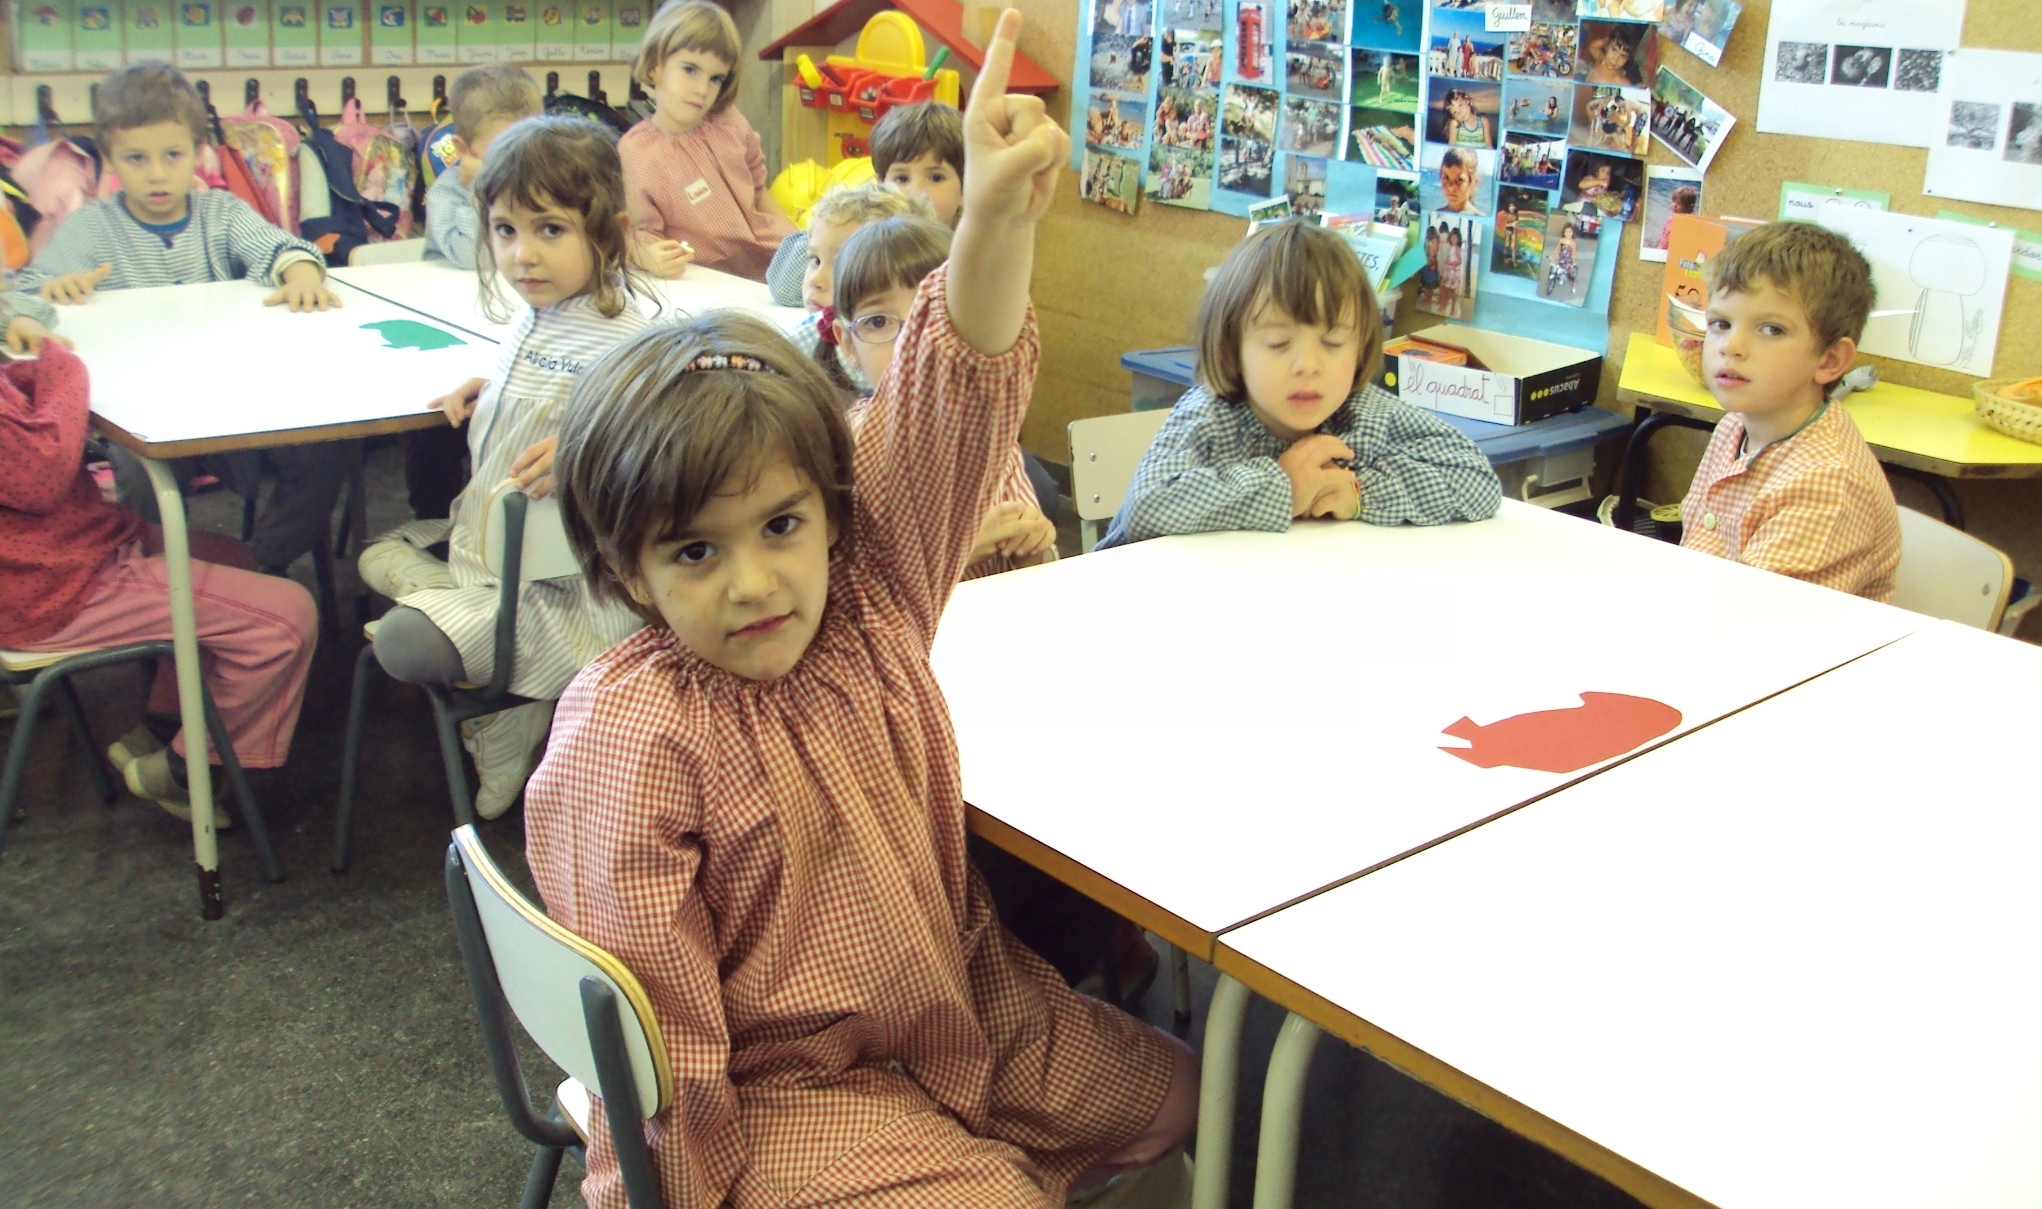
\includegraphics[width=18cm,keepaspectratio]{parvulari/img/foto3b.jpg}}
{Parvulari}
{21} %pagesof

Entenem com a hàbits aquelles situacions que es repeteixen de forma sistemàtica i ens ajuden a agafar seguretat i a poder preveure els fets.

També ens ajuden a estructurar-nos, a orientar-nos i a evolucionar millor.
Els bons hàbits també possibiliten una relació de convivència positiva amb tots i amb tot.

Quan més estructurats estiguem, més preparats estarem per la nostra autonomia personal. 

Els hàbits s’han de treballar a casa i a l’escola. A mida que anem assolint els diferents hàbits ens sentirem més segurs, tranquils i amb ganes d’aprendre.
Aprendre a observar els petits progressos que fa cadascú, dia a dia,  i saber valorar-los és per a la persona  una motivació important i necessària per continuar avançant.

Aquests  són alguns dels hàbits que aprenem a la classe de cargols, a la classe de pingüins i a la dels elefants.

Els cargols expliquen: hàbits d’autonomia
La Metis ens ensenya a rentar-nos les mans, abans ho fèiem  malament i no ens quedaven netes , ara ja ho fem bé perquè som grans .


\noindent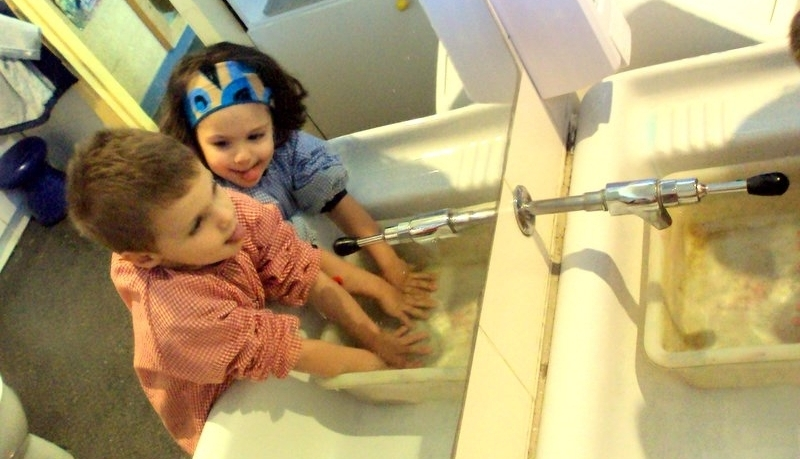
\includegraphics[width=9cm,keepaspectratio]{parvulari/img/foto1b.jpg}

També hem après a treure’ns la jaqueta i posar-nos la bata nosaltres solets i, quan no podem, ens ajuda la Metis i el Martí


\noindent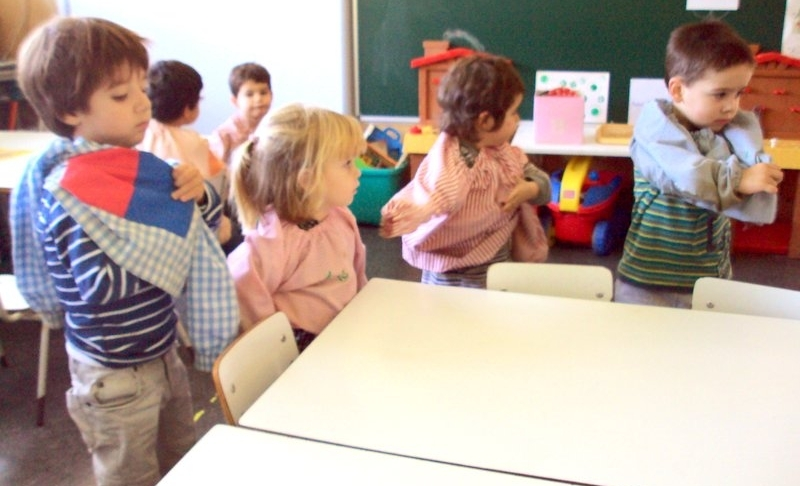
\includegraphics[width=9cm,keepaspectratio]{parvulari/img/foto2b.jpg}



Els pingüins expliquen: hàbits socials

A la classe dels pingüins,  la Rosa ens ensenya que quan volem dir una cosa  hem d’aixecar la mà i,  si hi ha moltes mans alçades, ens hem de saber esperar i no parlar tots alhora.



%\noindent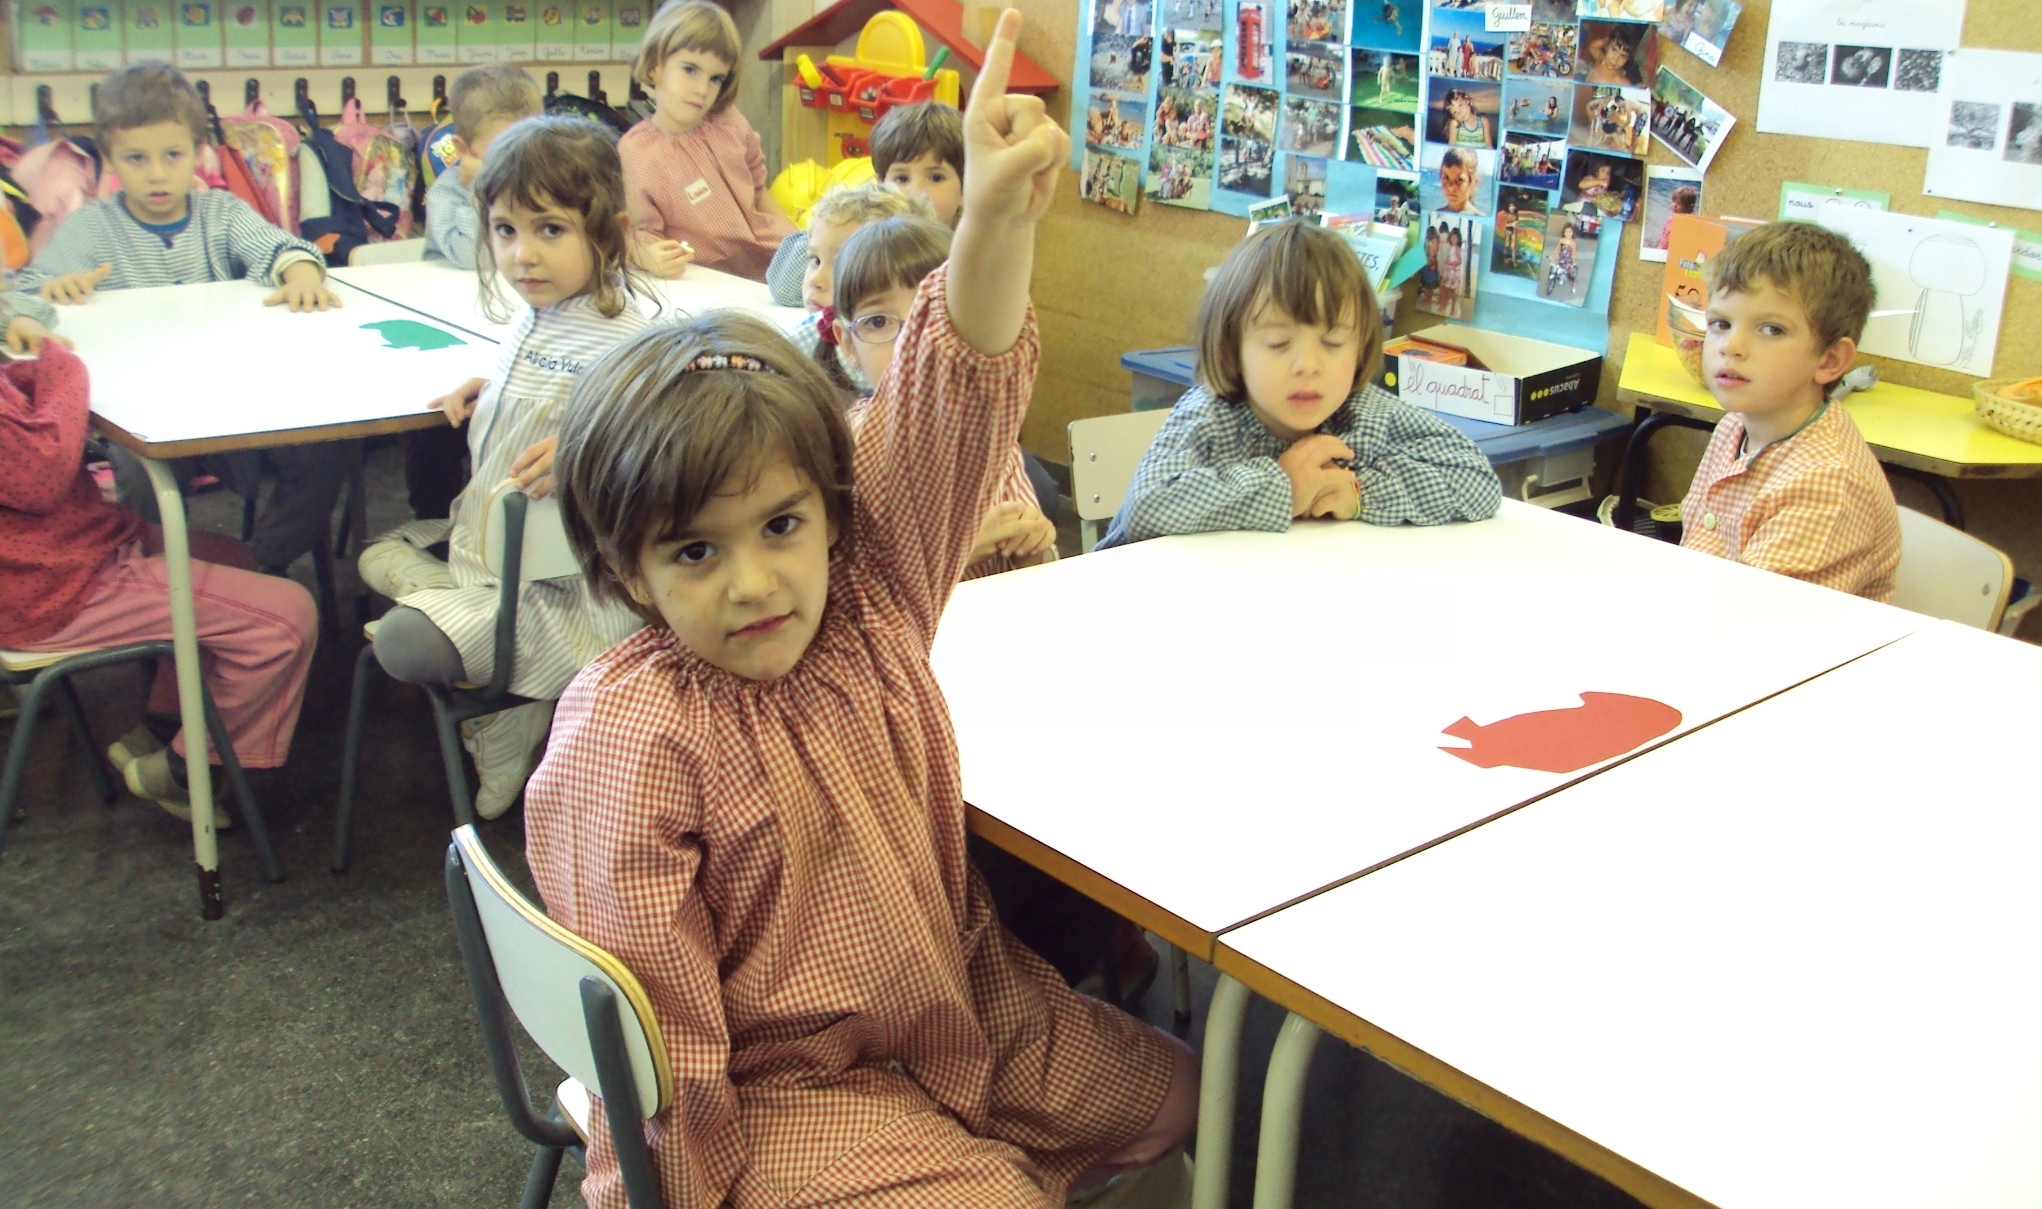
\includegraphics[width=9cm,keepaspectratio]{parvulari/img/foto3b.jpg}

Ara hem après a compartir les joguines,  a endreçar-les i a recollir les coses a poc a poc i respectant el material



\noindent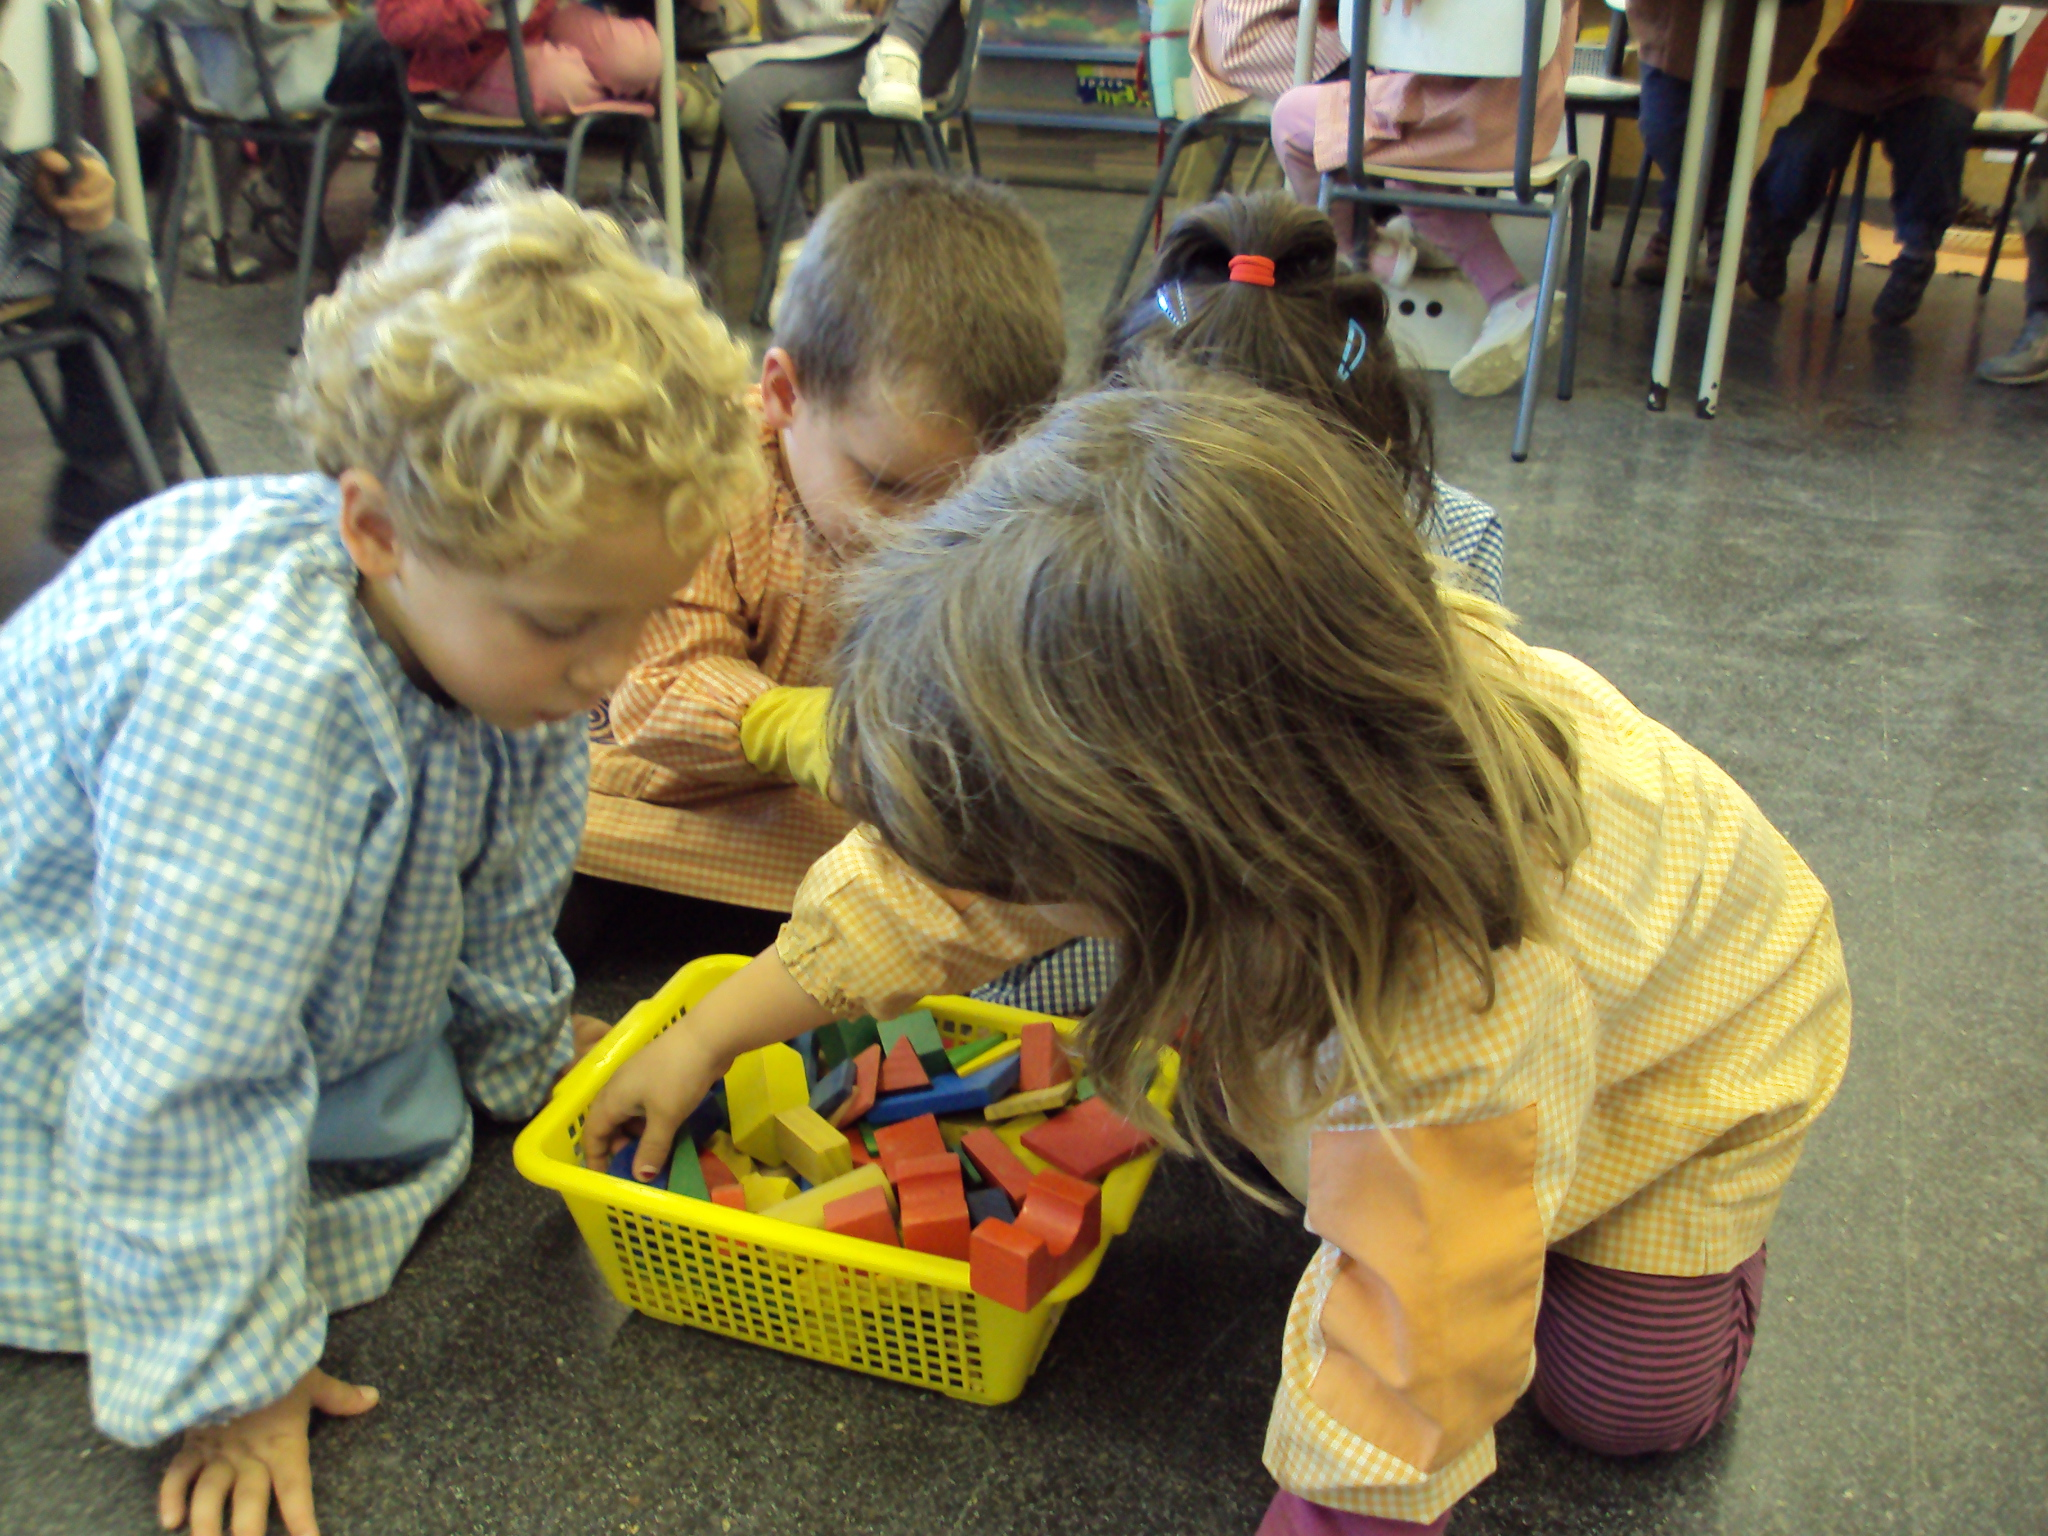
\includegraphics[width=9cm,keepaspectratio]{parvulari/img/foto4.jpg}

Els elefants expliquen: hàbits de treball

Nosaltres aprenem a escriure i a fer frases i la Toni ens posa deures per aprendre molt

\noindent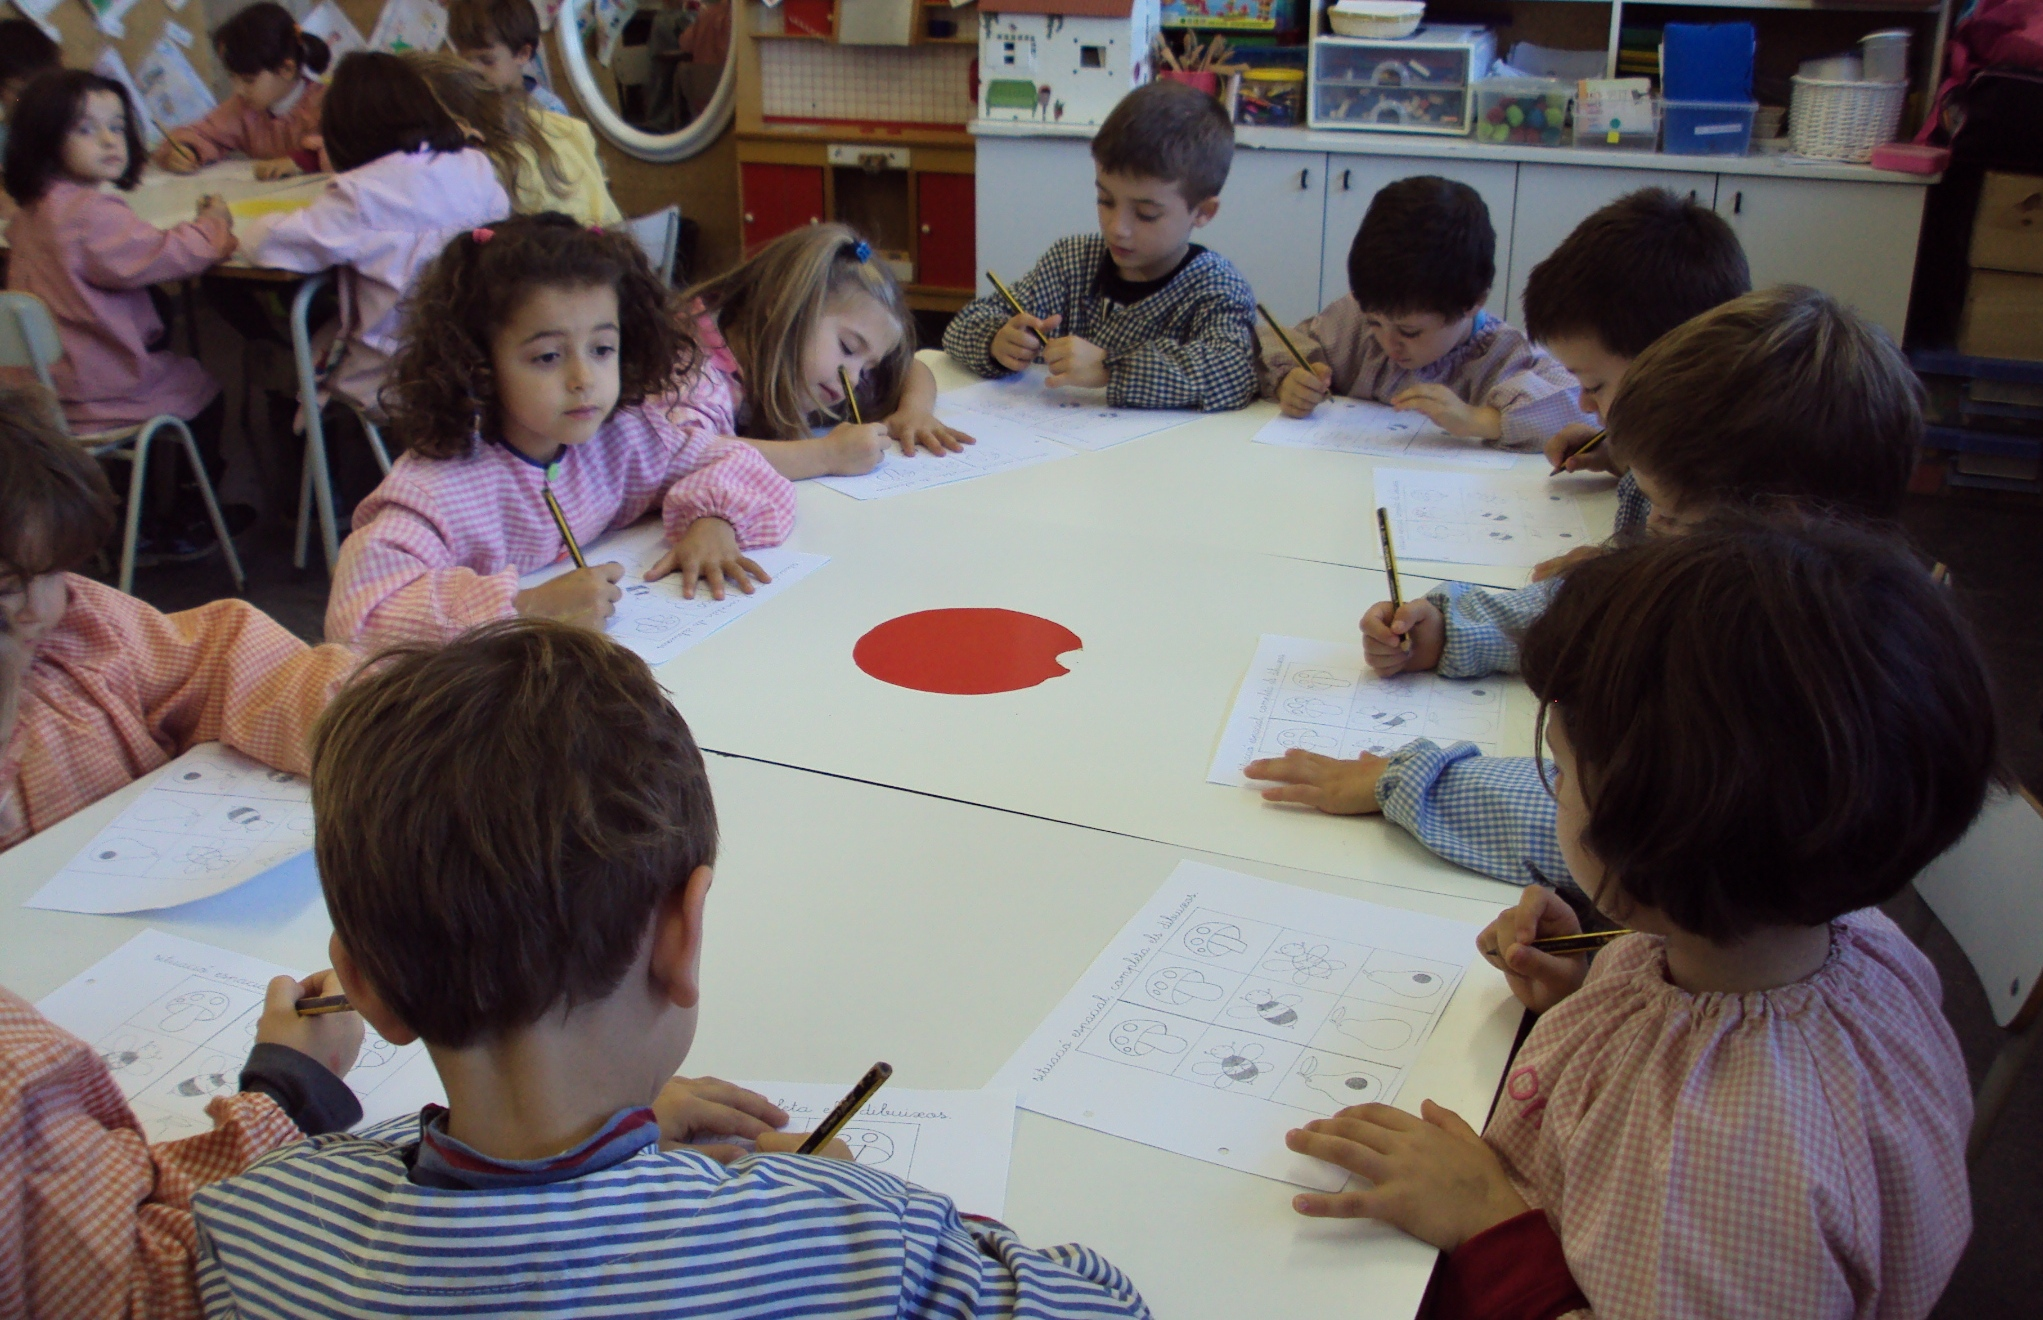
\includegraphics[width=9cm,keepaspectratio]{parvulari/img/foto5b.jpg}

Quan ens enfadem ara ja no ens barallem, parlem entre nosaltres perquè ja som molt grans

Fem quadern de matemàtiques, anem a l’aula d’informàtica i treballem amb la P.D.I.


\noindent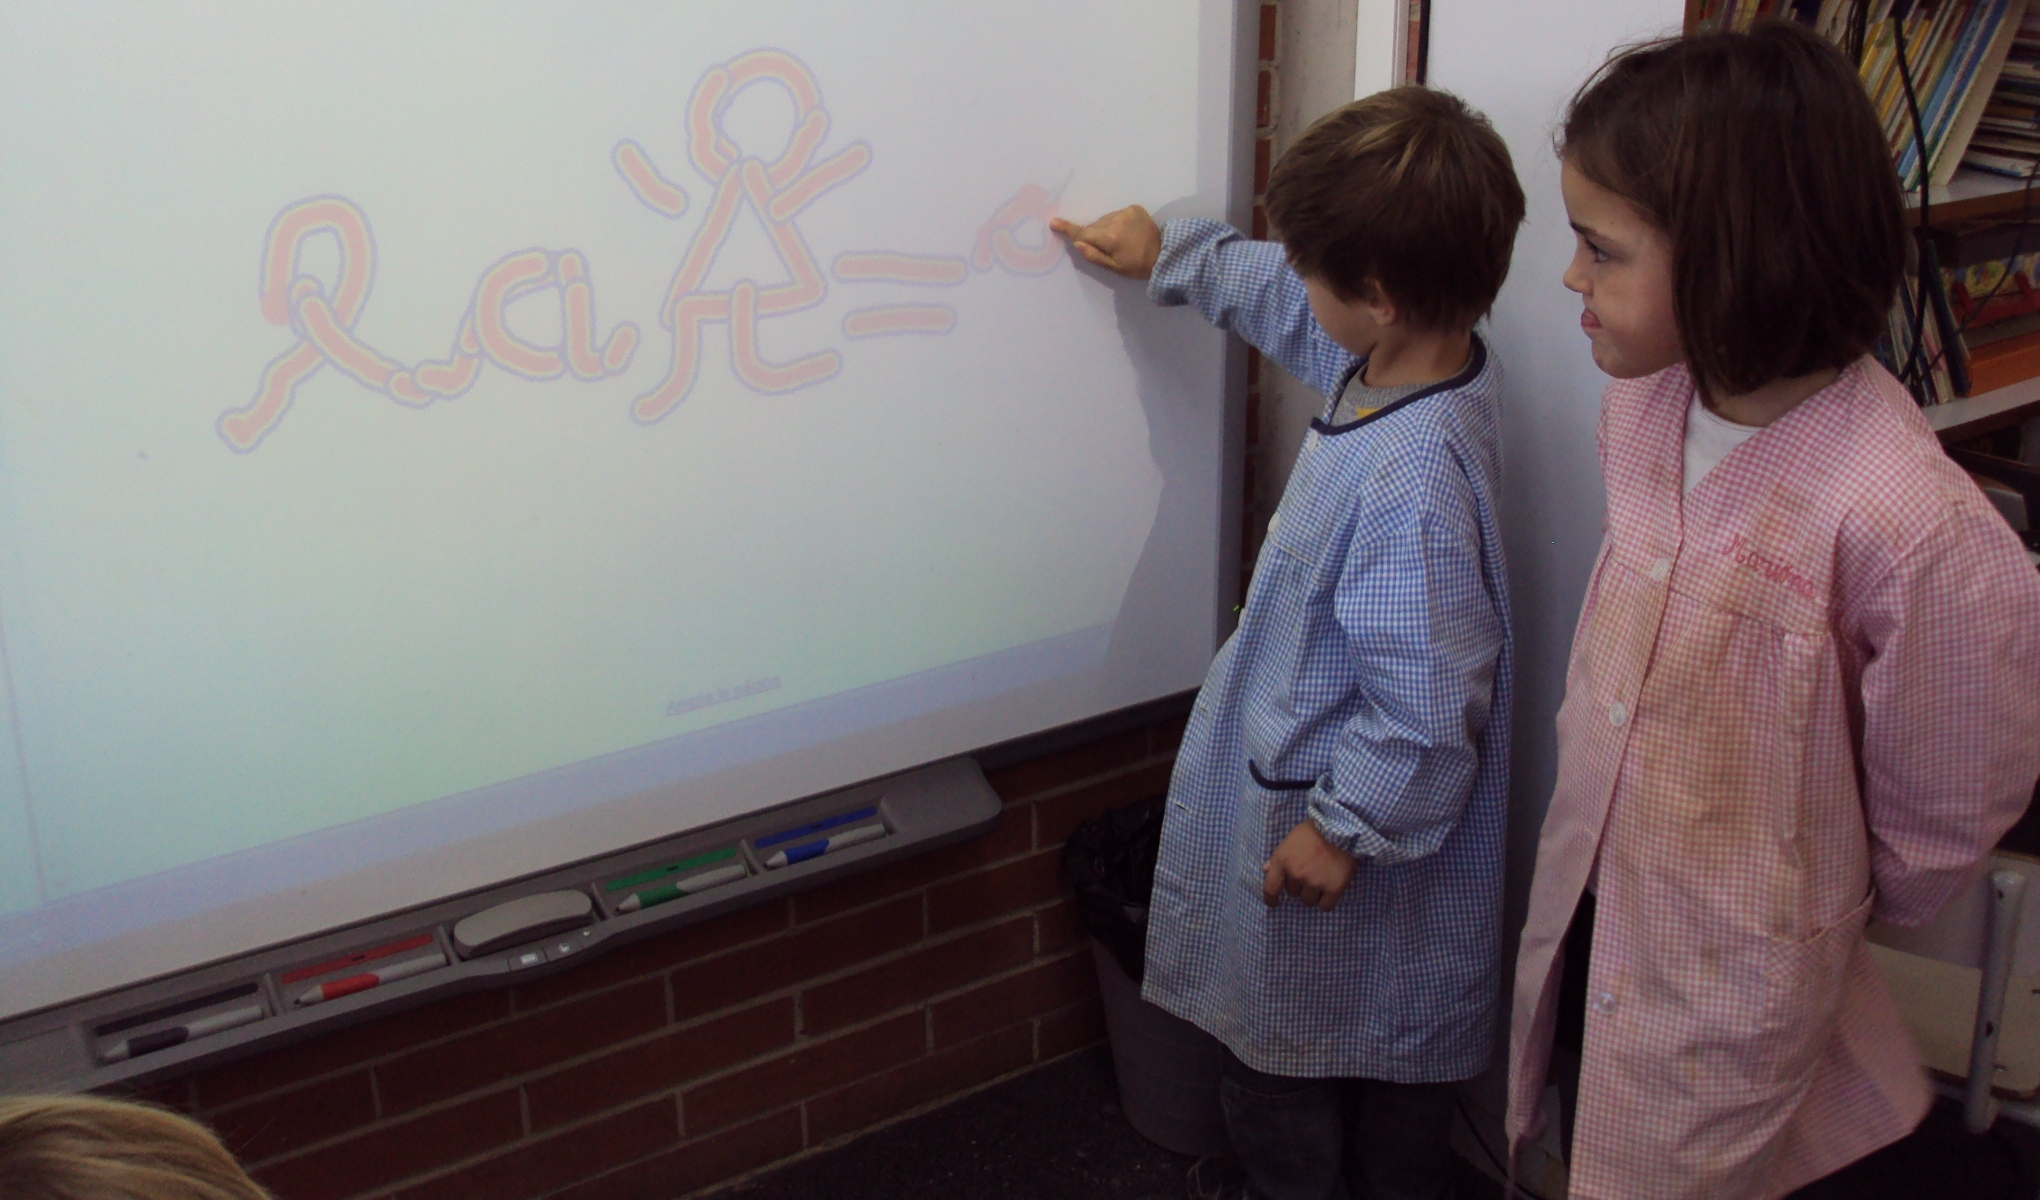
\includegraphics[width=9cm,keepaspectratio]{parvulari/img/foto6b.jpg}


Ara ja som grans i abans de contestar,  primer hem de pensar.


Tots aquests hàbits són  necessaris per a l’adquisició dels nous aprenentatges que assolirem al llarg de tota la nostra escolaritat.


\authorandplace{Les mestres de Parvulari}{Escola Solc}

\end{news}

\noindent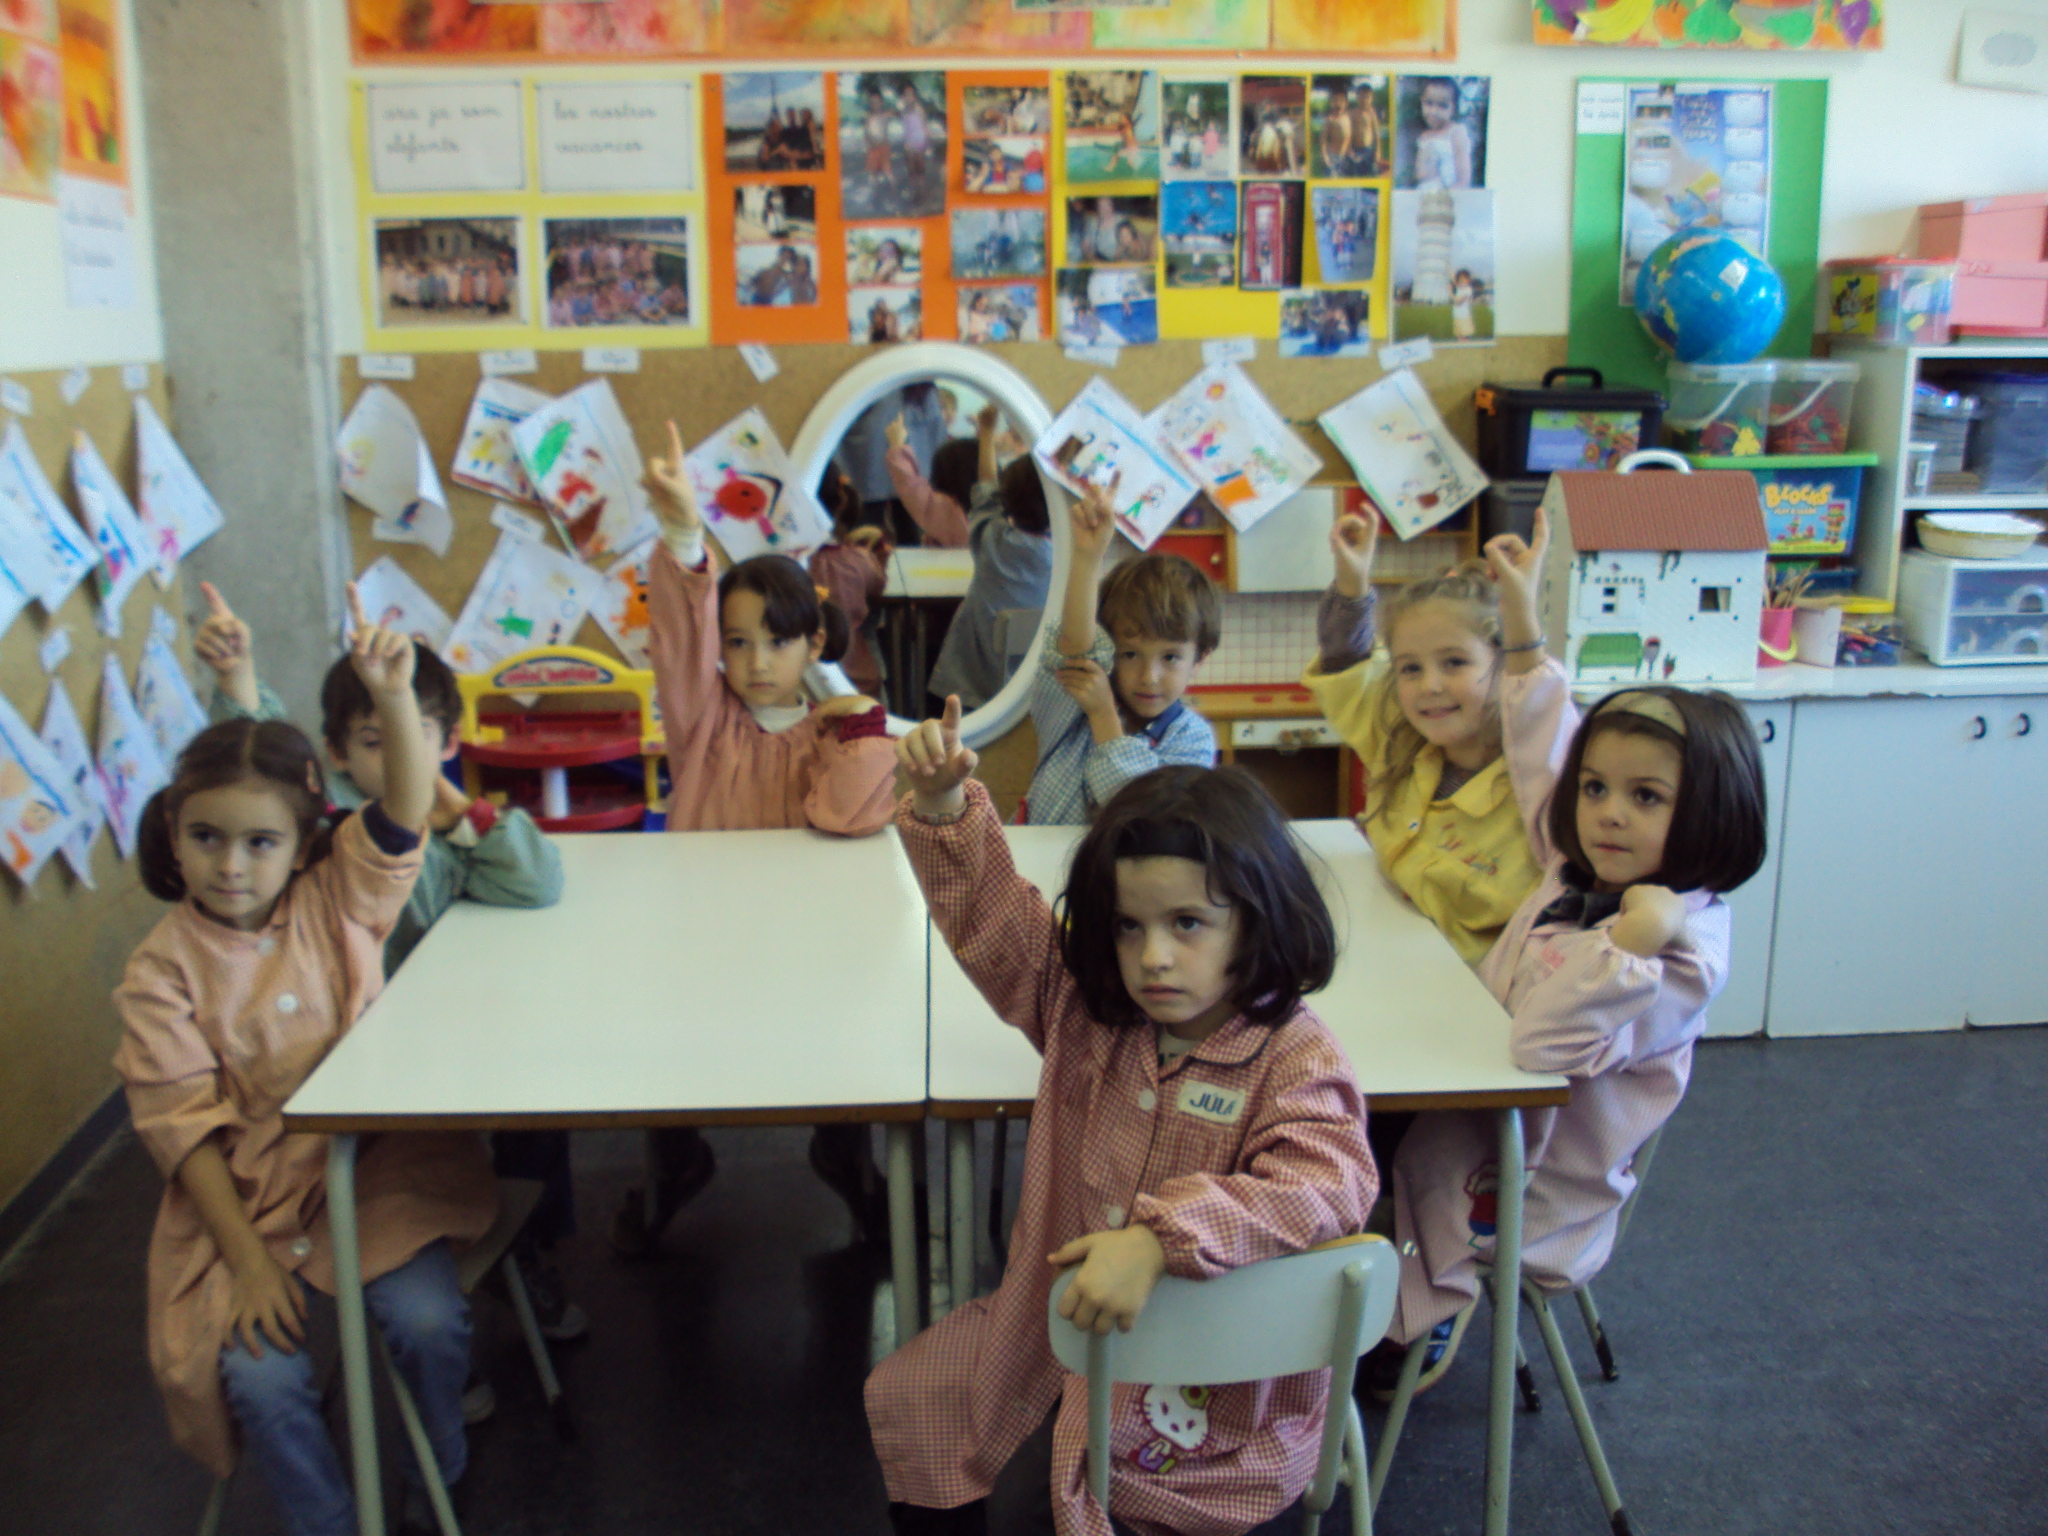
\includegraphics[width=12.5cm,keepaspectratio]{parvulari/img/foto7.jpg}
